\documentclass{standalone}

\usepackage[utf8]{inputenc}
\usepackage[OT1]{fontenc}

\usepackage{tikz}
\usetikzlibrary{arrows,shapes,positioning,shadows,trees}

\tikzset{
  basic/.style  = {draw, text width=2cm, drop shadow, font=\sffamily, rectangle},
  root/.style   = {basic, rounded corners=2pt, thin, align=center,
                   fill=white},
  level 2/.style = {basic, rounded corners=6pt, thin,align=center, fill=white, text width=2cm},
  level 3/.style = {basic, thin, align=left, fill=white, text width=2.8cm}
}

\newcommand{\distance}{25pt}

\begin{document}
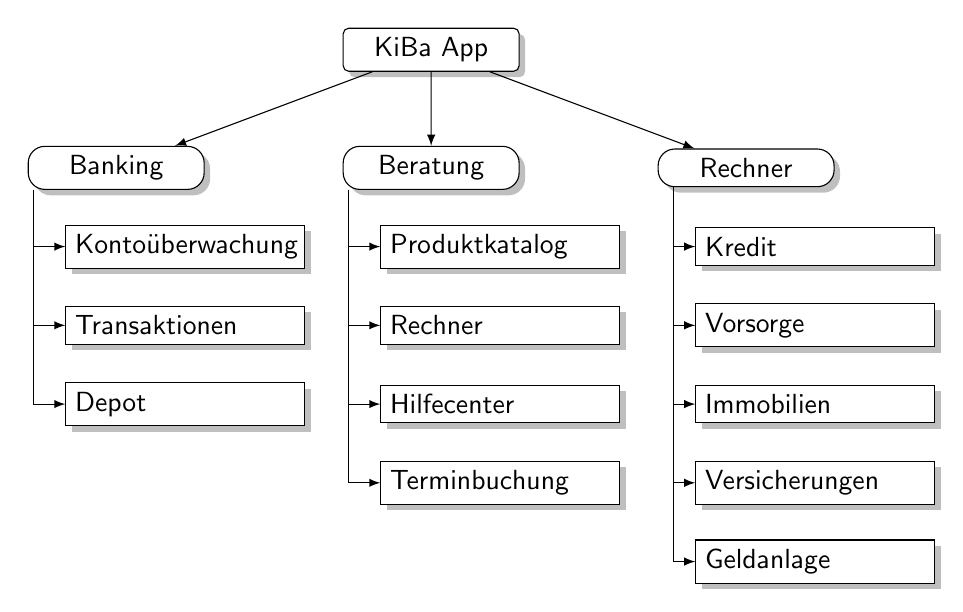
\begin{tikzpicture}[
  level 1/.style={sibling distance=40mm},
  edge from parent/.style={->,draw},
  >=latex]

% root of the the initial tree, level 1
\node[root] {KiBa App}
% The first level, as children of the initial tree
  child {node[level 2] (c1) {Banking}}
  child {node[level 2] (c2) {Beratung}}
  child {node[level 2] (c3) {Rechner}};

% The second level, relatively positioned nodes
\begin{scope}[every node/.style={level 3}]
\node [below of = c1, xshift=\distance] (c11) {Kontoüberwachung};
\node [below of = c11] (c12) {Transaktionen};
\node [below of = c12] (c13) {Depot};

\node [below of = c2, xshift=\distance] (c21) {Produktkatalog};
\node [below of = c21] (c22) {Rechner};
\node [below of = c22] (c23) {Hilfecenter};
\node [below of = c23] (c24) {Terminbuchung};

\node [below of = c3, xshift=\distance] (c31) {Kredit};
\node [below of = c31] (c32) {Vorsorge};
\node [below of = c32] (c33) {Immobilien};
\node [below of = c33] (c34) {Versicherungen};
\node [below of = c34] (c35) {Geldanlage};
\end{scope}

% lines from each level 1 node to every one of its "children"
\foreach \value in {1,2,3}
  \draw[->] (c1.195) |- (c1\value.west);

\foreach \value in {1,...,4}
  \draw[->] (c2.195) |- (c2\value.west);

\foreach \value in {1,...,5}
  \draw[->] (c3.195) |- (c3\value.west);
\end{tikzpicture}
\end{document}